\documentclass[tikz,border=0pt]{standalone}
\usepackage{xcolor}
\usetikzlibrary{calc}
% Palette: Sam_Comm_final.png by eye, and data/palette.json.
\definecolor{ink}{HTML}{3B2340}
\definecolor{sky}{HTML}{EFC46A}
\definecolor{skyhi}{HTML}{F5DA92}
\definecolor{skylow}{HTML}{E9B060}
\definecolor{cloud}{HTML}{F2D58A}
\definecolor{wallA}{HTML}{E88A73}
\definecolor{wallB}{HTML}{EE9F7E}
\definecolor{wallC}{HTML}{E47A7E}
\definecolor{wallD}{HTML}{F0B07E}
\definecolor{wallE}{HTML}{D9765F}
\definecolor{wallF}{HTML}{E99A8A}
\definecolor{greenA}{HTML}{8DBB7E}
\definecolor{greenB}{HTML}{6FA77A}
\definecolor{greenC}{HTML}{A9C97F}
\definecolor{greenD}{HTML}{5E9C6A}
\definecolor{window}{HTML}{F6E7A0}
\definecolor{windark}{HTML}{8C5A64}
\definecolor{metal}{HTML}{8D9A93}
\definecolor{metaldark}{HTML}{5E6B66}
\definecolor{wood}{HTML}{B9835A}
\definecolor{paving}{HTML}{E2BD8C}
\definecolor{ground}{HTML}{D3A77D}
\definecolor{stone}{HTML}{E7C9A0}
\definecolor{clock}{HTML}{F8EBC8}
\definecolor{court}{HTML}{9E4F55}
\definecolor{courtdark}{HTML}{6E3542}
\definecolor{goldtrim}{HTML}{F2B53A}
\definecolor{paper}{HTML}{F6E7C4}
\definecolor{paperdark}{HTML}{E3CC98}
\definecolor{violet}{HTML}{7B2FF7}
\definecolor{magenta}{HTML}{FF2E88}
\definecolor{cyan}{HTML}{13CFE3}
\definecolor{gold}{HTML}{FFB000}
\definecolor{coat}{HTML}{2F4858}
\definecolor{coatdark}{HTML}{22323F}
\definecolor{trim}{HTML}{F26B38}
\definecolor{skin}{HTML}{E0AC69}
\definecolor{hair}{HTML}{3B2340}
\definecolor{gun}{HTML}{3E3A46}
\definecolor{robe}{HTML}{2D2240}
\definecolor{bossface}{HTML}{F8EBC8}
\definecolor{eye}{HTML}{FF2E88}
\definecolor{red}{HTML}{B3262E}
\definecolor{heart}{HTML}{FF4F6D}
\definecolor{jump}{HTML}{8DE36B}
\definecolor{lamp}{HTML}{FFE6A3}
\definecolor{night}{HTML}{4A3357}
\definecolor{nightsky}{HTML}{6B4A6E}
% One ink for every outline (the TikZ house style and the game's ink pass).
\newcommand{\Ink}{1.1pt}
\tikzset{inked/.style={draw=ink, line width=\Ink, line join=round, line cap=round}}
\begin{document}
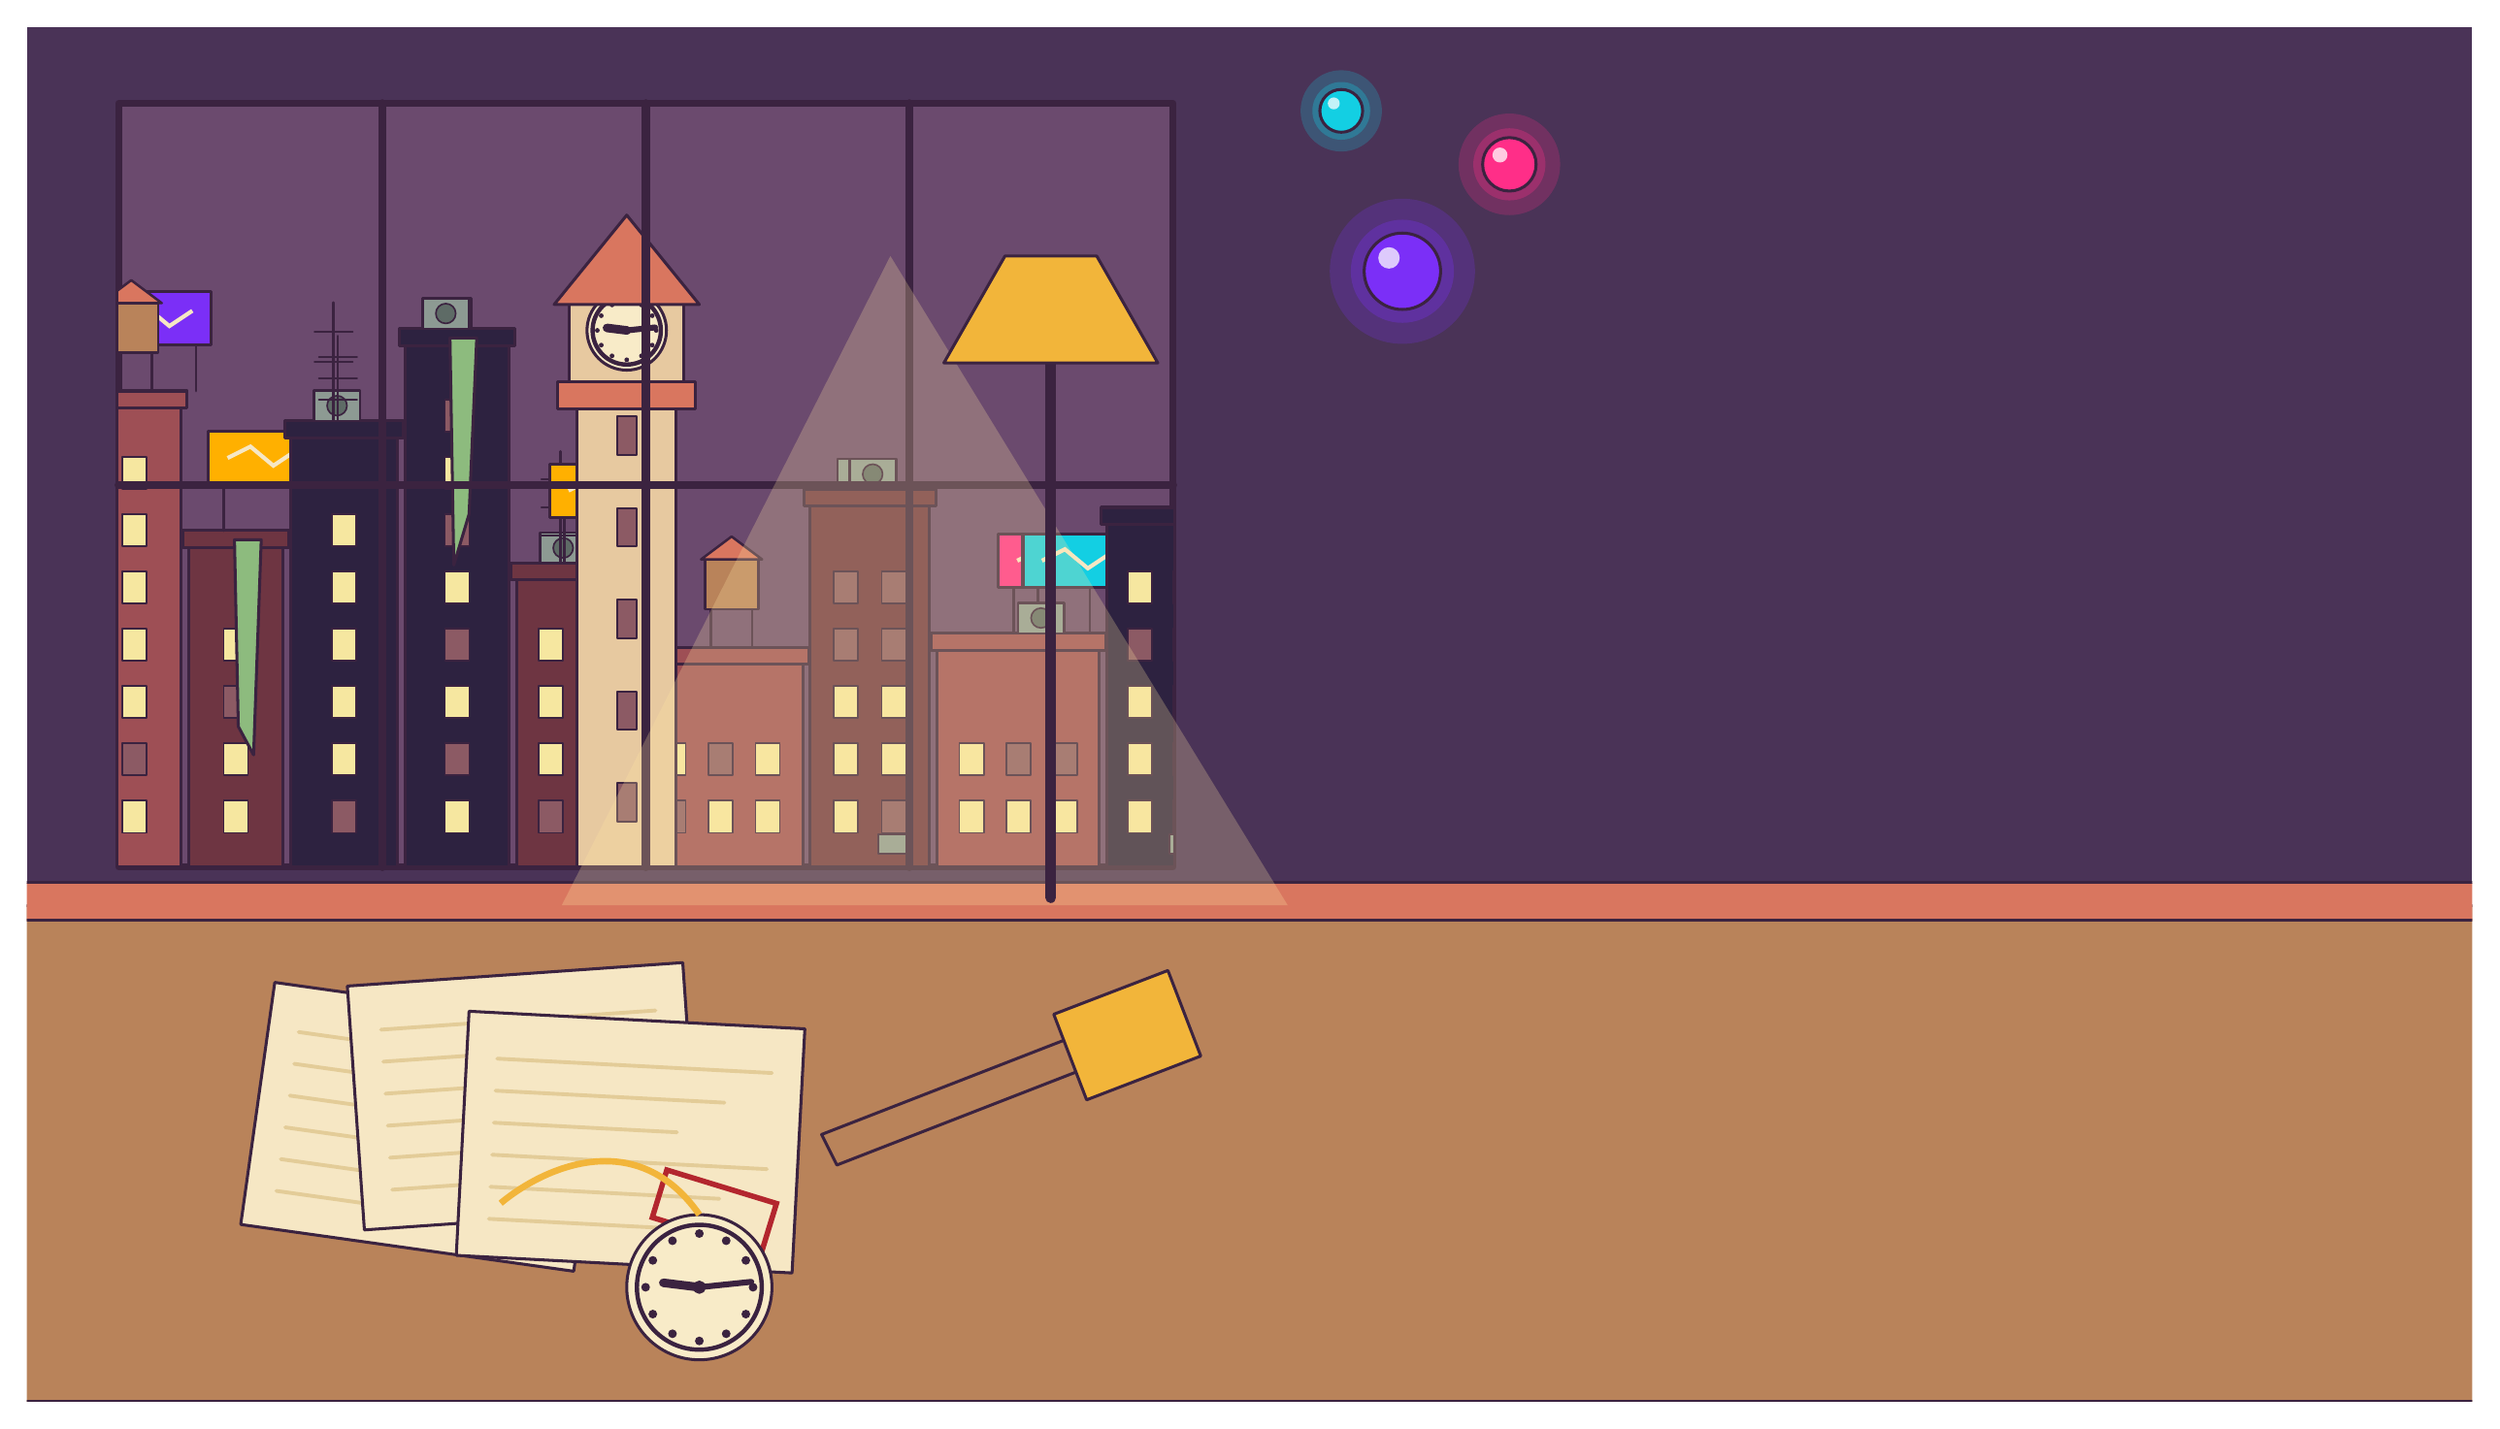
\begin{tikzpicture}
\clip (0,0) rectangle (32,18);
\fill[night] (0,0) rectangle (32,18);
\filldraw[inked,line width=2.5pt,fill=nightsky] (1.2,7) rectangle (15,17);
\begin{scope}\clip (1.2,7.0) rectangle (15.0,17.0);
\filldraw[inked,fill=court] (0.8,7) rectangle (2.018,13.013);
\filldraw[inked,fill=court] (0.72,13.013) rectangle (2.098,13.233);
\filldraw[inked,line width=0.6pt,fill=window] (1.249,7.45) rectangle (1.569,7.87);
\filldraw[inked,line width=0.6pt,fill=windark] (1.249,8.2) rectangle (1.569,8.62);
\filldraw[inked,line width=0.6pt,fill=window] (1.249,8.95) rectangle (1.569,9.37);
\filldraw[inked,line width=0.6pt,fill=window] (1.249,9.7) rectangle (1.569,10.12);
\filldraw[inked,line width=0.6pt,fill=window] (1.249,10.45) rectangle (1.569,10.87);
\filldraw[inked,line width=0.6pt,fill=window] (1.249,11.2) rectangle (1.569,11.62);
\filldraw[inked,line width=0.6pt,fill=window] (1.249,11.95) rectangle (1.569,12.37);
\draw[ink, line width=1pt, line cap=round] (1.215,13.233) -- (1.215,13.833);
\draw[ink, line width=1pt, line cap=round] (2.215,13.233) -- (2.215,13.833);
\filldraw[inked,fill=violet] (1.015,13.833) rectangle (2.415,14.533);
\draw[paper, line width=1.5pt] (1.265,14.183) -- (1.565,14.333) -- (1.865,14.083) -- (2.165,14.283);
\draw[ink, line width=0.9pt, line cap=round] (1.096,13.233) -- (1.096,13.733);
\draw[ink, line width=0.9pt, line cap=round] (1.636,13.233) -- (1.636,13.733);
\filldraw[inked,line width=0.9pt,fill=wood] (1.016,13.733) rectangle (1.716,14.383);
\filldraw[inked,fill=wallE,line width=0.9pt] (0.966,14.383) -- (1.766,14.383) -- (1.366,14.683) -- cycle;
\filldraw[inked,fill=courtdark] (2.118,7) rectangle (3.353,11.185);
\filldraw[inked,fill=courtdark] (2.038,11.185) rectangle (3.433,11.405);
\filldraw[inked,line width=0.6pt,fill=window] (2.575,7.45) rectangle (2.895,7.87);
\filldraw[inked,line width=0.6pt,fill=window] (2.575,8.2) rectangle (2.895,8.62);
\filldraw[inked,line width=0.6pt,fill=windark] (2.575,8.95) rectangle (2.895,9.37);
\filldraw[inked,line width=0.6pt,fill=window] (2.575,9.7) rectangle (2.895,10.12);
\draw[ink, line width=1pt, line cap=round] (2.576,11.405) -- (2.576,12.005);
\draw[ink, line width=1pt, line cap=round] (3.576,11.405) -- (3.576,12.005);
\filldraw[inked,fill=gold] (2.376,12.005) rectangle (3.776,12.705);
\draw[paper, line width=1.5pt] (2.626,12.355) -- (2.926,12.505) -- (3.226,12.255) -- (3.526,12.455);
\filldraw[inked,fill=greenA] (2.717,11.285) -- (3.067,11.285) -- (2.967,8.469) -- (2.767,8.841) -- cycle;
\filldraw[inked,fill=robe] (3.453,7) rectangle (4.851,12.621);
\filldraw[inked,fill=robe] (3.373,12.621) rectangle (4.931,12.841);
\filldraw[inked,line width=0.6pt,fill=windark] (3.992,7.45) rectangle (4.312,7.87);
\filldraw[inked,line width=0.6pt,fill=window] (3.992,8.2) rectangle (4.312,8.62);
\filldraw[inked,line width=0.6pt,fill=window] (3.992,8.95) rectangle (4.312,9.37);
\filldraw[inked,line width=0.6pt,fill=window] (3.992,9.7) rectangle (4.312,10.12);
\filldraw[inked,line width=0.6pt,fill=window] (3.992,10.45) rectangle (4.312,10.87);
\filldraw[inked,line width=0.6pt,fill=window] (3.992,11.2) rectangle (4.312,11.62);
\filldraw[inked,line width=0.9pt,fill=metal] (3.759,12.841) rectangle (4.359,13.241);
\filldraw[inked,fill=metaldark,line width=0.6pt] (4.059,13.041) circle (0.13);
\draw[ink, line width=0.9pt, line cap=round] (4.014,12.841) -- (4.014,14.392);
\draw[ink, line width=0.7pt, line cap=round] (3.764,13.229) -- (4.264,13.229);
\draw[ink, line width=0.7pt, line cap=round] (3.764,13.616) -- (4.264,13.616);
\draw[ink, line width=0.7pt, line cap=round] (3.764,14.004) -- (4.264,14.004);
\draw[ink, line width=0.9pt, line cap=round] (4.071,12.841) -- (4.071,13.954);
\draw[ink, line width=0.7pt, line cap=round] (3.821,13.119) -- (4.321,13.119);
\draw[ink, line width=0.7pt, line cap=round] (3.821,13.397) -- (4.321,13.397);
\draw[ink, line width=0.7pt, line cap=round] (3.821,13.676) -- (4.321,13.676);
\filldraw[inked,fill=robe] (4.951,7) rectangle (6.311,13.827);
\filldraw[inked,fill=robe] (4.871,13.827) rectangle (6.391,14.047);
\filldraw[inked,line width=0.6pt,fill=window] (5.471,7.45) rectangle (5.791,7.87);
\filldraw[inked,line width=0.6pt,fill=windark] (5.471,8.2) rectangle (5.791,8.62);
\filldraw[inked,line width=0.6pt,fill=window] (5.471,8.95) rectangle (5.791,9.37);
\filldraw[inked,line width=0.6pt,fill=windark] (5.471,9.7) rectangle (5.791,10.12);
\filldraw[inked,line width=0.6pt,fill=window] (5.471,10.45) rectangle (5.791,10.87);
\filldraw[inked,line width=0.6pt,fill=windark] (5.471,11.2) rectangle (5.791,11.62);
\filldraw[inked,line width=0.6pt,fill=window] (5.471,11.95) rectangle (5.791,12.37);
\filldraw[inked,line width=0.6pt,fill=windark] (5.471,12.7) rectangle (5.791,13.12);
\filldraw[inked,line width=0.9pt,fill=metal] (5.213,14.047) rectangle (5.813,14.447);
\filldraw[inked,fill=metaldark,line width=0.6pt] (5.513,14.247) circle (0.13);
\filldraw[inked,line width=0.9pt,fill=metal] (5.182,14.047) rectangle (5.782,14.447);
\filldraw[inked,fill=metaldark,line width=0.6pt] (5.482,14.247) circle (0.13);
\filldraw[inked,fill=greenA] (5.537,13.927) -- (5.887,13.927) -- (5.787,11.621) -- (5.587,10.955) -- cycle;
\filldraw[inked,fill=courtdark] (6.411,7) rectangle (7.905,10.758);
\filldraw[inked,fill=courtdark] (6.331,10.758) rectangle (7.985,10.978);
\filldraw[inked,line width=0.6pt,fill=windark] (6.695,7.45) rectangle (7.015,7.87);
\filldraw[inked,line width=0.6pt,fill=window] (6.695,8.2) rectangle (7.015,8.62);
\filldraw[inked,line width=0.6pt,fill=window] (6.695,8.95) rectangle (7.015,9.37);
\filldraw[inked,line width=0.6pt,fill=window] (6.695,9.7) rectangle (7.015,10.12);
\filldraw[inked,line width=0.6pt,fill=window] (7.3,7.45) rectangle (7.62,7.87);
\filldraw[inked,line width=0.6pt,fill=windark] (7.3,8.2) rectangle (7.62,8.62);
\filldraw[inked,line width=0.7pt,fill=metal] (7.25,7.92) rectangle (7.67,8.18);
\filldraw[inked,line width=0.6pt,fill=windark] (7.3,8.95) rectangle (7.62,9.37);
\filldraw[inked,line width=0.6pt,fill=windark] (7.3,9.7) rectangle (7.62,10.12);
\filldraw[inked,line width=0.9pt,fill=metal] (6.718,10.978) rectangle (7.318,11.378);
\filldraw[inked,fill=metaldark,line width=0.6pt] (7.018,11.178) circle (0.13);
\draw[ink, line width=0.9pt, line cap=round] (6.983,10.978) -- (6.983,12.443);
\draw[ink, line width=0.7pt, line cap=round] (6.733,11.344) -- (7.233,11.344);
\draw[ink, line width=0.7pt, line cap=round] (6.733,11.711) -- (7.233,11.711);
\draw[ink, line width=0.7pt, line cap=round] (6.733,12.077) -- (7.233,12.077);
\draw[ink, line width=1pt, line cap=round] (7.038,10.978) -- (7.038,11.578);
\draw[ink, line width=1pt, line cap=round] (8.038,10.978) -- (8.038,11.578);
\filldraw[inked,fill=gold] (6.838,11.578) rectangle (8.238,12.278);
\draw[paper, line width=1.5pt] (7.088,11.928) -- (7.388,12.078) -- (7.688,11.828) -- (7.988,12.028);
\filldraw[inked,fill=court] (8.005,7) rectangle (10.152,9.658);
\filldraw[inked,fill=court] (7.925,9.658) rectangle (10.232,9.878);
\filldraw[inked,line width=0.6pt,fill=windark] (8.302,7.45) rectangle (8.622,7.87);
\filldraw[inked,line width=0.6pt,fill=window] (8.302,8.2) rectangle (8.622,8.62);
\filldraw[inked,line width=0.6pt,fill=window] (8.919,7.45) rectangle (9.239,7.87);
\filldraw[inked,line width=0.6pt,fill=windark] (8.919,8.2) rectangle (9.239,8.62);
\filldraw[inked,line width=0.6pt,fill=window] (9.535,7.45) rectangle (9.855,7.87);
\filldraw[inked,line width=0.6pt,fill=window] (9.535,8.2) rectangle (9.855,8.62);
\draw[ink, line width=0.9pt, line cap=round] (8.952,9.878) -- (8.952,10.378);
\draw[ink, line width=0.9pt, line cap=round] (9.492,9.878) -- (9.492,10.378);
\filldraw[inked,line width=0.9pt,fill=wood] (8.872,10.378) rectangle (9.572,11.028);
\filldraw[inked,fill=wallE,line width=0.9pt] (8.822,11.028) -- (9.622,11.028) -- (9.222,11.328) -- cycle;
\filldraw[inked,fill=courtdark] (10.252,7) rectangle (11.813,11.724);
\filldraw[inked,fill=courtdark] (10.172,11.724) rectangle (11.893,11.944);
\filldraw[inked,line width=0.6pt,fill=window] (10.559,7.45) rectangle (10.879,7.87);
\filldraw[inked,line width=0.6pt,fill=window] (10.559,8.2) rectangle (10.879,8.62);
\filldraw[inked,line width=0.6pt,fill=window] (10.559,8.95) rectangle (10.879,9.37);
\filldraw[inked,line width=0.6pt,fill=windark] (10.559,9.7) rectangle (10.879,10.12);
\filldraw[inked,line width=0.6pt,fill=windark] (10.559,10.45) rectangle (10.879,10.87);
\filldraw[inked,line width=0.6pt,fill=windark] (11.186,7.45) rectangle (11.506,7.87);
\filldraw[inked,line width=0.7pt,fill=metal] (11.136,7.17) rectangle (11.556,7.43);
\filldraw[inked,line width=0.6pt,fill=window] (11.186,8.2) rectangle (11.506,8.62);
\filldraw[inked,line width=0.6pt,fill=window] (11.186,8.95) rectangle (11.506,9.37);
\filldraw[inked,line width=0.6pt,fill=windark] (11.186,9.7) rectangle (11.506,10.12);
\filldraw[inked,line width=0.6pt,fill=windark] (11.186,10.45) rectangle (11.506,10.87);
\filldraw[inked,line width=0.9pt,fill=metal] (10.784,11.944) rectangle (11.384,12.344);
\filldraw[inked,fill=metaldark,line width=0.6pt] (11.084,12.144) circle (0.13);
\filldraw[inked,line width=0.9pt,fill=metal] (10.606,11.944) rectangle (11.206,12.344);
\filldraw[inked,fill=metaldark,line width=0.6pt] (10.906,12.144) circle (0.13);
\filldraw[inked,line width=0.9pt,fill=metal] (10.768,11.944) rectangle (11.368,12.344);
\filldraw[inked,fill=metaldark,line width=0.6pt] (11.068,12.144) circle (0.13);
\filldraw[inked,fill=court] (11.913,7) rectangle (14.037,9.841);
\filldraw[inked,fill=court] (11.833,9.841) rectangle (14.117,10.061);
\filldraw[inked,line width=0.6pt,fill=window] (12.204,7.45) rectangle (12.524,7.87);
\filldraw[inked,line width=0.6pt,fill=window] (12.204,8.2) rectangle (12.524,8.62);
\filldraw[inked,line width=0.6pt,fill=window] (12.815,7.45) rectangle (13.135,7.87);
\filldraw[inked,line width=0.6pt,fill=windark] (12.815,8.2) rectangle (13.135,8.62);
\filldraw[inked,line width=0.6pt,fill=window] (13.426,7.45) rectangle (13.746,7.87);
\filldraw[inked,line width=0.6pt,fill=windark] (13.426,8.2) rectangle (13.746,8.62);
\draw[ink, line width=1pt, line cap=round] (12.91,10.061) -- (12.91,10.661);
\draw[ink, line width=1pt, line cap=round] (13.91,10.061) -- (13.91,10.661);
\filldraw[inked,fill=magenta] (12.71,10.661) rectangle (14.11,11.361);
\draw[paper, line width=1.5pt] (12.96,11.011) -- (13.26,11.161) -- (13.56,10.911) -- (13.86,11.111);
\draw[ink, line width=1pt, line cap=round] (13.234,10.061) -- (13.234,10.661);
\draw[ink, line width=1pt, line cap=round] (14.234,10.061) -- (14.234,10.661);
\filldraw[inked,fill=cyan] (13.034,10.661) rectangle (14.434,11.361);
\draw[paper, line width=1.5pt] (13.284,11.011) -- (13.584,11.161) -- (13.884,10.911) -- (14.184,11.111);
\filldraw[inked,line width=0.9pt,fill=metal] (12.971,10.061) rectangle (13.571,10.461);
\filldraw[inked,fill=metaldark,line width=0.6pt] (13.271,10.261) circle (0.13);
\filldraw[inked,fill=robe] (14.137,7) rectangle (16.178,11.489);
\filldraw[inked,fill=robe] (14.057,11.489) rectangle (16.258,11.709);
\filldraw[inked,line width=0.6pt,fill=window] (14.407,7.45) rectangle (14.727,7.87);
\filldraw[inked,line width=0.6pt,fill=window] (14.407,8.2) rectangle (14.727,8.62);
\filldraw[inked,line width=0.6pt,fill=window] (14.407,8.95) rectangle (14.727,9.37);
\filldraw[inked,line width=0.6pt,fill=windark] (14.407,9.7) rectangle (14.727,10.12);
\filldraw[inked,line width=0.6pt,fill=window] (14.407,10.45) rectangle (14.727,10.87);
\filldraw[inked,line width=0.6pt,fill=windark] (14.998,7.45) rectangle (15.318,7.87);
\filldraw[inked,line width=0.7pt,fill=metal] (14.948,7.17) rectangle (15.368,7.43);
\filldraw[inked,line width=0.6pt,fill=windark] (14.998,8.2) rectangle (15.318,8.62);
\filldraw[inked,line width=0.6pt,fill=window] (14.998,8.95) rectangle (15.318,9.37);
\filldraw[inked,line width=0.6pt,fill=windark] (14.998,9.7) rectangle (15.318,10.12);
\filldraw[inked,line width=0.6pt,fill=windark] (14.998,10.45) rectangle (15.318,10.87);
\filldraw[inked,line width=0.6pt,fill=windark] (15.588,7.45) rectangle (15.908,7.87);
\filldraw[inked,line width=0.6pt,fill=window] (15.588,8.2) rectangle (15.908,8.62);
\filldraw[inked,line width=0.6pt,fill=window] (15.588,8.95) rectangle (15.908,9.37);
\filldraw[inked,line width=0.6pt,fill=windark] (15.588,9.7) rectangle (15.908,10.12);
\filldraw[inked,line width=0.6pt,fill=windark] (15.588,10.45) rectangle (15.908,10.87);
\filldraw[inked,line width=0.9pt,fill=metal] (15.003,11.709) rectangle (15.603,12.109);
\filldraw[inked,fill=metaldark,line width=0.6pt] (15.303,11.909) circle (0.13);
\filldraw[inked,fill=stone] (7.2,7) rectangle (8.5,13);
\filldraw[inked,fill=wallE] (6.95,13) rectangle (8.75,13.35);
\filldraw[inked,fill=stone] (7.1,13.35) rectangle (8.6,14.365);
\filldraw[inked,fill=clock] (7.85,14.026) circle (0.52);
\draw[ink, line width=1.6pt] (7.85,14.026) circle (0.447);
\foreach \k in {0,...,11} { \fill[ink] ($(7.85,14.026)+(\k*30:0.385)$) circle (0.031); }
\draw[ink, line width=3.2pt, line cap=round] (7.85,14.026) -- (7.592,14.058);
\draw[ink, line width=2.2pt, line cap=round] (7.85,14.026) -- (8.222,14.065);
\filldraw[inked,fill=ink] (7.85,14.026) circle (0.036);
\filldraw[inked,fill=wallE] (6.9,14.365) -- (8.8,14.365) -- (7.85,15.535) -- cycle;
\filldraw[inked,line width=0.7pt,fill=windark] (7.72,7.6) rectangle (7.98,8.1);
\filldraw[inked,line width=0.7pt,fill=windark] (7.72,8.8) rectangle (7.98,9.3);
\filldraw[inked,line width=0.7pt,fill=windark] (7.72,10) rectangle (7.98,10.5);
\filldraw[inked,line width=0.7pt,fill=windark] (7.72,11.2) rectangle (7.98,11.7);
\filldraw[inked,line width=0.7pt,fill=windark] (7.72,12.4) rectangle (7.98,12.9);
\end{scope}
\draw[ink, line width=3pt, line cap=round] (4.65,7) -- (4.65,17);
\draw[ink, line width=3pt, line cap=round] (8.1,7) -- (8.1,17);
\draw[ink, line width=3pt, line cap=round] (11.55,7) -- (11.55,17);
\draw[ink, line width=3pt, line cap=round] (1.2,12) -- (15,12);
\filldraw[inked,fill=wood] (-0.5,0) -- (32.5,0) -- (32.5,6.5) -- (-0.5,6.5) -- cycle;
\filldraw[inked,fill=wallE] (-0.5,6.3) rectangle (32.5,6.8);
\begin{scope}[rotate around={-8:(5.2,3.6)}]
\filldraw[inked,fill=paper] (3,2) rectangle (7.4,5.2);
\draw[paperdark, line width=1.4pt, line cap=round] (3.4,4.6) -- (7,4.6);
\draw[paperdark, line width=1.4pt, line cap=round] (3.4,4.18) -- (6.4,4.18);
\draw[paperdark, line width=1.4pt, line cap=round] (3.4,3.76) -- (5.8,3.76);
\draw[paperdark, line width=1.4pt, line cap=round] (3.4,3.34) -- (7,3.34);
\draw[paperdark, line width=1.4pt, line cap=round] (3.4,2.92) -- (6.4,2.92);
\draw[paperdark, line width=1.4pt, line cap=round] (3.4,2.5) -- (5.8,2.5);
\draw[red, line width=2pt, rotate around={-14:(6.3,2.8)}] (5.6,2.45) rectangle (7.1,3.1);
\end{scope}
\begin{scope}[rotate around={4:(6.5,4)}]
\filldraw[inked,fill=paper] (4.3,2.4) rectangle (8.7,5.6);
\draw[paperdark, line width=1.4pt, line cap=round] (4.7,5) -- (8.3,5);
\draw[paperdark, line width=1.4pt, line cap=round] (4.7,4.58) -- (7.7,4.58);
\draw[paperdark, line width=1.4pt, line cap=round] (4.7,4.16) -- (7.1,4.16);
\draw[paperdark, line width=1.4pt, line cap=round] (4.7,3.74) -- (8.3,3.74);
\draw[paperdark, line width=1.4pt, line cap=round] (4.7,3.32) -- (7.7,3.32);
\draw[paperdark, line width=1.4pt, line cap=round] (4.7,2.9) -- (7.1,2.9);
\draw[red, line width=2pt, rotate around={-14:(7.6,3.2)}] (6.9,2.85) rectangle (8.4,3.5);
\end{scope}
\begin{scope}[rotate around={-3:(7.9,3.4)}]
\filldraw[inked,fill=paper] (5.7,1.8) rectangle (10.1,5);
\draw[paperdark, line width=1.4pt, line cap=round] (6.1,4.4) -- (9.7,4.4);
\draw[paperdark, line width=1.4pt, line cap=round] (6.1,3.98) -- (9.1,3.98);
\draw[paperdark, line width=1.4pt, line cap=round] (6.1,3.56) -- (8.5,3.56);
\draw[paperdark, line width=1.4pt, line cap=round] (6.1,3.14) -- (9.7,3.14);
\draw[paperdark, line width=1.4pt, line cap=round] (6.1,2.72) -- (9.1,2.72);
\draw[paperdark, line width=1.4pt, line cap=round] (6.1,2.3) -- (8.5,2.3);
\draw[red, line width=2pt, rotate around={-14:(9,2.6)}] (8.3,2.25) rectangle (9.8,2.9);
\end{scope}
\filldraw[inked,fill=wood] (10.6,3.1) -- (14.2,4.5) -- (14,4.9) -- (10.4,3.5) -- cycle;
\filldraw[inked,fill=goldtrim,rotate around={21:(14.4,4.8)}] (13.6,4.2) rectangle (15.2,5.4);
\fill[lamp, opacity=0.25] (11.3,15.0) -- (7.0,6.5) -- (16.5,6.5) -- cycle;
\draw[ink, line width=4pt, line cap=round] (13.4,6.6) -- (13.4,13.8);
\filldraw[inked,fill=goldtrim] (12,13.6) -- (14.8,13.6) -- (14,15) -- (12.8,15) -- cycle;
\filldraw[inked,fill=clock] (8.8,1.5) circle (0.95);
\draw[ink, line width=1.6pt] (8.8,1.5) circle (0.817);
\foreach \k in {0,...,11} { \fill[ink] ($(8.8,1.5)+(\k*30:0.703)$) circle (0.057); }
\draw[ink, line width=3.2pt, line cap=round] (8.8,1.5) -- (8.329,1.558);
\draw[ink, line width=2.2pt, line cap=round] (8.8,1.5) -- (9.48,1.571);
\filldraw[inked,fill=ink] (8.8,1.5) circle (0.067);
\draw[goldtrim, line width=2.4pt] (8.8,2.45) .. controls (8.0,3.6) and (6.8,3.1) .. (6.2,2.6);
\fill[violet, opacity=0.22] (18,14.8) circle (0.95);
\fill[violet, opacity=0.3] (18,14.8) circle (0.675);
\filldraw[inked,fill=violet] (18,14.8) circle (0.5);
\fill[white, opacity=0.75] (17.825,14.975) circle (0.14);
\fill[magenta, opacity=0.22] (19.4,16.2) circle (0.665);
\fill[magenta, opacity=0.3] (19.4,16.2) circle (0.472);
\filldraw[inked,fill=magenta] (19.4,16.2) circle (0.35);
\fill[white, opacity=0.75] (19.277,16.322) circle (0.098);
\fill[cyan, opacity=0.22] (17.2,16.9) circle (0.532);
\fill[cyan, opacity=0.3] (17.2,16.9) circle (0.378);
\filldraw[inked,fill=cyan] (17.2,16.9) circle (0.28);
\fill[white, opacity=0.75] (17.102,16.998) circle (0.078);
\end{tikzpicture}
\end{document}
